%==============================================================================
%== template for LATEX poster =================================================
%==============================================================================
%
%--A0 beamer slide-------------------------------------------------------------
\documentclass[final]{beamer}
\usepackage{etex} % too many packages in beamerposter
\usepackage[orientation=portrait,size=a0,
            scale=1.25         % font scale factor
           ]{beamerposter}
          
\usepackage{booktabs}
\geometry{
  hmargin=2.5cm, % little modification of margins
}

%
\usepackage[utf8]{inputenc}
\graphicspath{{figures/}} % Location of the graphics files
\newcommand{\abnet}{{\sc ABnet}}
\newcommand{\norm}[1]{\lVert#1\rVert}
\newcommand{\tup}[1]{\langle#1\rangle}

\linespread{1.05} %%% TODO CHANGE (was 1.15)
%
%==The poster style============================================================
\usetheme{sharelatex}

%==Title, date and authors of the poster=======================================
\title
[Interspeech (2015, Dresden, Germany)] % Conference
{ % Poster title
Hybrid Spoken Term Discovery-ABnet System\\
Finding words to learn segments
}

\author{ % Authors
Roland Thiolli\`ere\inst{*}, Ewan Dunbar\inst{*}, Gabriel Synnaeve\inst{*\dagger}, Maarten Versteegh\inst{*}, Emmanuel Dupoux\inst{*}
}
\institute
[ENS] % General University
{
\inst{*} LSCP, \'{E}cole Normale Sup\'{e}rieure / EHESS / CNRS, Paris, France\\%[0.3ex]
\inst{\dagger} now at Facebook AI Research\\[0.5ex]
\inst{} \begin{small}\texttt{rolthiolliere@gmail.com, emd@umd.edu, gabrielsynnaeve@gmail.com, maartenversteegh@gmail.com, emmanuel.dupoux@gmail.com}\end{small}
}
%\date{\today}


\begin{document}
\begin{frame}[t]
%==============================================================================
\begin{multicols}{3} % try 2
%==============================================================================
%==The poster content==========================================================
%==============================================================================

\section{Introduction}

\begin{itemize}
\item This system is the combination of two architectures: a spoken term discovery\cite{jansenvandurme2011} (STD) and a siamese neural network\cite{synnaevedupoux2014} (\abnet{}).
\item The STD system find matching patterns in the acoustic signal.
\item The \abnet{} is train to minimize the distance between those matching patterns, and maximize the distance between non matching patterns.
\end{itemize}


%-----------------------------------------
%	Motivation
%-----------------------------------------

\section{Motivation}

\begin{itemize}
\item The high level idea: that two randomly selected words are more distant in the acoustic space than two randomly selected phonemes. It is easier to discriminate words than phonemes.
\item Our approach: extract word level information to learn phonemes.
\end{itemize}

%-----------------------------------------
%       SYSTEM
%-----------------------------------------

\section{System}

\begin{figure}[ht!]
  \begin{center}
    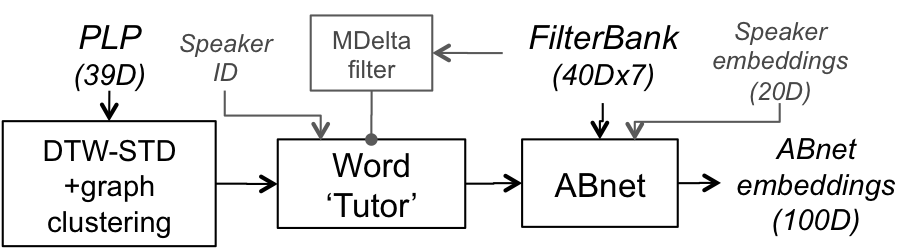
\includegraphics[width=0.85\columnwidth]{System2.png}
    \caption{\label{fig:system}Overview of the components of our system.}
  \end{center}
\end{figure}

%-----------------------------------------
%       SPOKEN TERM DISCOVERY
%-----------------------------------------

\subsection{Spoken term discovery}

\begin{itemize}
\item System used as baseline for track 2\cite{versteeghetal2015}
\item Finding patterns in an approximation of the similarity matrix.
\item Computes an approximation of the similarity matrix (cosine similarity).
\item Searches for diagonal patterns in that matrix.
\item Those matching patterns are then filtered and clustered.
\end{itemize}

This is only a succinct description of the system and there is a lot more to it.

\begin{figure}[ht!]
  \begin{center}
    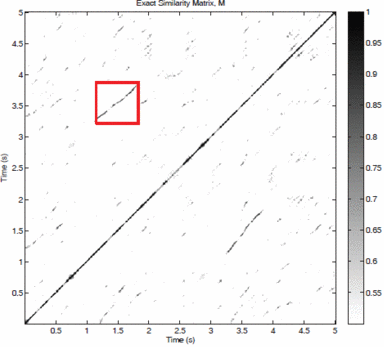
\includegraphics[width=0.85\columnwidth]{similarity_matrix}
    \caption{\label{fig:system}Similarity matrix of the signal.}
  \end{center}
\end{figure}

\subsection{Word tutor}

The word tutor selects the words that it will feed to the \abnet{}, making the link between the STD system and the \abnet{}.
Pairs of ``different'' words are randomly selected amongst the discovered patterns. All pairs of words (same and different) are DTW aligned.

We extract 40 dimensionnal log-energy Mel-scale filterbanks (10ms step and 25ms window size). 7 adjacent (following the ``aligned'' path) frames are stacked as input for the \abnet{}.

\subsection{ABnet}

\begin{itemize}
\item The \abnet{} is a siamese neural network architecture: the weights in the second branch are the duplicate of the weights in the first branch.
\item Input: a pair of examples (A, B) and a label Y=(same|different)
\item loss function = similarity if same, distance if different.

\begin{figure}[ht!]
  \begin{center}
    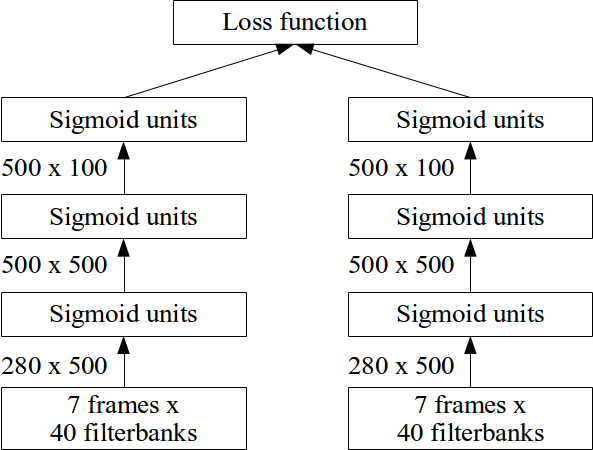
\includegraphics[width=0.85\columnwidth]{abnet_cropped.png}
    \caption{\label{fig:system}Overview of the components of our system.}
  \end{center}
\end{figure}

\item Loss function used:

\[
\mathcal{L}(A, B) =
\begin{cases}
(1-\cos(Y_A, Y_B)) / 2 & \text{if same} \\
\cos^2(Y_A, Y_B)       & \text{if different}
\end{cases}
\]

\noindent        
where $$\cos(x, y) = \frac{\tup{x, y}}{\norm{x}\norm{y}}$$

\item It learns a space where inputs with the same label are close together, and inputs with different labels are far appart. 
\end{itemize}

%-----------------------------------------
%	Extensions
%-----------------------------------------

\section*{Extensions}

We investigate the use of temporal information, and speaker information.

\subsection{Mdelta}

Adding temporal information.


\begin{figure}[ht!]
  \begin{center}
    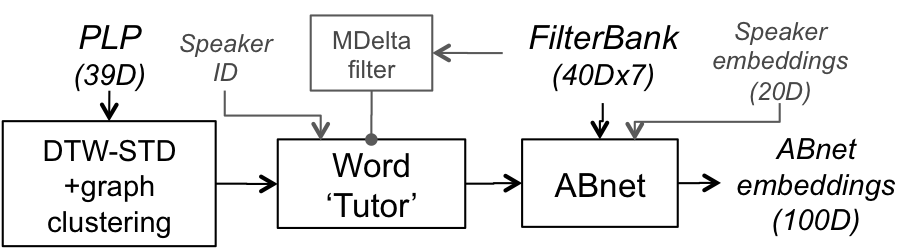
\includegraphics[width=0.85\columnwidth]{System2.png}
    \caption{\label{fig:system}Overview of the components of our system.}
  \end{center}
\end{figure}

\subsection*{Speaker embedding}

Adding speaker information.


\begin{figure}[ht!]
  \begin{center}
    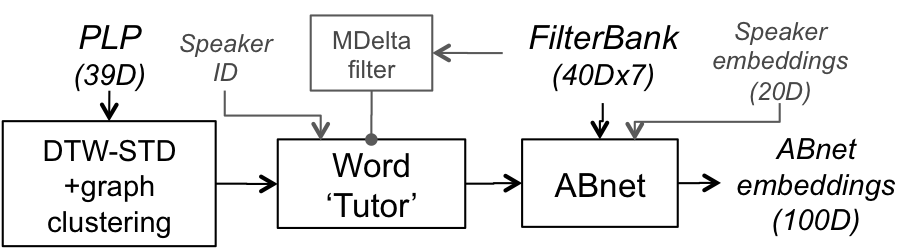
\includegraphics[width=\columnwidth]{System2.png}
    \caption{\label{fig:system}Overview of the components of our system.}
  \end{center}
\end{figure}


%----------------------------------------------------------------------------------------
%	RESULTS 
%----------------------------------------------------------------------------------------

\section{Results}

The speech representation is evaluated with the ABX paradigm\cite{versteeghetal2015}.

The overall system raised a substancial improvement over baseline.

%
\begin{table}[htb]
\caption{ Within and across speaker Minimal Pair ABX error rates for the ZeroSpeech baseline (MFCC) and topline (supervised HMM-GMM posteriorgrams), and for our systems.}
\label{tab:track1}
\vspace{1cm}
\centerline{
\begin{tabular}{lcccc}
\hline
\vspace{1cm}        & \multicolumn{2}{c}{\underline{English}}  & \multicolumn{2}{c}{\underline{Xitsonga}}    \\
                        & Within  & Across   & Within  & Across   \\
\hline
Baseline (MFCC)          & \emph{15.6}      & \emph{28.1}      & \emph{19.1}      & \emph{33.8}      \\
Topline (HMM-GMM)           & \emph{12.1}      & \emph{16.0}      & \emph{3.5}       & \emph{4.5}      \\
\hline
STD $\rightarrow$ \abnet{} & \textbf{12.0}      & \textbf{17.9}      & \textbf{11.7}      & \textbf{16.6}      \\
STD / MDF $\rightarrow$ \abnet{} & 12.4      & 18.1      & 12.6      & 18.6      \\
STD + SpkID $\rightarrow$ \abnet{} & 12.2      & 18.0      & 16.5      & 21.3      \\
\hline
\end{tabular}
}
\end{table}
%


\begin{table}[h]
\caption{\label{tab:std-stats} Output of the spoken term discovery system. These fragments (``words'') serve as input to the \abnet{}.}
\small
% \begin{tabular}{lccccccccccccccccc}
\begin{tabular}{lccccc}
\hline
         & Words & Pairs & Classes & NED   & Coverage \\
\hline
Engl.~E(1,3) & 6512 & 4305 & 3149 & 0.219 & 0.163 \\
Engl.~E(2) & 4334 & 2630 & 2092 & 0.229 & 0.106 \\
Xits.~E(1,3) & 3582 & 1818 & 1782 & 0.120 & 0.162 \\
Xits.~E(2) & 2286 & 1158 & 1138 &  0.105 & 0.106 \\
\hline
\end{tabular}
\end{table}

%----------------------------------------------------------------------------------------
%	CONCLUSIONS
%----------------------------------------------------------------------------------------

% \color{SaddleBrown} % SaddleBrown color for the conclusions to make them stand out

\section{Conclusions}

The results validate the approach. Despite the low number of examples, a good speech representation can be learnt.\\
However, all our attempts to further improve the results by adding additional information failed.

% \color{DarkSlateGray} % Set the color back to DarkSlateGray for the rest of the content

%----------------------------------------------------------------------------------------
%	FORTHCOMING RESEARCH
%----------------------------------------------------------------------------------------

\section{Forthcoming Research}

\begin{itemize}
\item Loop over the system (STD on learnt features).
\item Succesfully apply MDelta to STD output to improve track 2.
\end{itemize}

%----------------------------------------------------------------------------------------
%	REFERENCES
%----------------------------------------------------------------------------------------

\nocite{*} % Print all references regardless of whether they were cited in the poster or not
\bibliographystyle{IEEEtran} % Plain referencing style
\bibliography{bib} % Use the example bibliography file sample.bib

%----------------------------------------------------------------------------------------
%	ACKNOWLEDGEMENTS
%----------------------------------------------------------------------------------------

\section{Acknowledgements}

This work really was a team effort, all authors contributed equally.\\
We would like to thank Aren Jensen for letting us use his spoken term discovery system pre-release, and for his technical support.
%----------------------------------------------------------------------------------------

%--End of references-----------------------------------------------------------

\end{multicols}

%==============================================================================
\end{frame}
\end{document}

